\documentclass{article}
%%%%%%%%%%%%%%%%%%%%%%%%%%%%%%%%%%%%%%%%%%%%%%%%%%%%%%%%%%%%%%%%%%%%%%%%%%%%%%%

%%%%%%%%%%%%%%%%%%%%%%%%%%%%% Using Packages %%%%%%%%%%%%%%%%%%%%%%%%%%%%%%%%%%
\usepackage{geometry}
\usepackage{graphicx}
\usepackage{amssymb}
\usepackage{amsmath}
\usepackage{amsthm}
\usepackage{empheq}
\usepackage{mdframed}
\usepackage{booktabs}
\usepackage{lipsum}
\usepackage{graphicx}
\usepackage{color}
\usepackage{psfrag}
\usepackage{pgfplots}
\usepackage{bm}
\usepackage{cancel}
\usepackage{multicol}
%%%%%%%%%%%%%%%%%%%%%%%%%%%%%%%%%%%%%%%%%%%%%%%%%%%%%%%%%%%%%%%%%%%%%%%%%%%%%%%

% Other Settings

%%%%%%%%%%%%%%%%%%%%%%%%%% Page Setting %%%%%%%%%%%%%%%%%%%%%%%%%%%%%%%%%%%%%%%
\geometry{a4paper}

%%%%%%%%%%%%%%%%%%%%%%%%%% Define some useful colors %%%%%%%%%%%%%%%%%%%%%%%%%%
\definecolor{ocre}{RGB}{243,102,25}
\definecolor{mygray}{RGB}{243,243,244}
\definecolor{deepGreen}{RGB}{26,111,0}
\definecolor{shallowGreen}{RGB}{235,255,255}
\definecolor{deepBlue}{RGB}{61,124,222}
\definecolor{shallowBlue}{RGB}{235,249,255}
%%%%%%%%%%%%%%%%%%%%%%%%%%%%%%%%%%%%%%%%%%%%%%%%%%%%%%%%%%%%%%%%%%%%%%%%%%%%%%%

%%%%%%%%%%%%%%%%%%%%%%%%%% Define an orangebox command %%%%%%%%%%%%%%%%%%%%%%%%
\newcommand\orangebox[1]{\fcolorbox{ocre}{mygray}{\hspace{1em}#1\hspace{1em}}}
%%%%%%%%%%%%%%%%%%%%%%%%%%%%%%%%%%%%%%%%%%%%%%%%%%%%%%%%%%%%%%%%%%%%%%%%%%%%%%%

%%%%%%%%%%%%%%%%%%%%%%%%%%%% English Environments %%%%%%%%%%%%%%%%%%%%%%%%%%%%%
\newtheoremstyle{mytheoremstyle}{3pt}{3pt}{\normalfont}{0cm}{\rmfamily\bfseries}{}{1em}{{\color{black}\thmname{#1}~\thmnumber{#2}}\thmnote{\,--\,#3}}
\newtheoremstyle{myproblemstyle}{3pt}{3pt}{\normalfont}{0cm}{\rmfamily\bfseries}{}{1em}{{\color{black}\thmname{#1}~\thmnumber{#2}}\thmnote{\,--\,#3}}
\theoremstyle{mytheoremstyle}
\newmdtheoremenv[linewidth=1pt,backgroundcolor=shallowGreen,linecolor=deepGreen,leftmargin=0pt,innerleftmargin=20pt,innerrightmargin=20pt,]{theorem}{Theorem}[section]
\theoremstyle{mytheoremstyle}
\newmdtheoremenv[linewidth=1pt,backgroundcolor=shallowBlue,linecolor=deepBlue,leftmargin=0pt,innerleftmargin=20pt,innerrightmargin=20pt,]{definition}{Definition}[section]
\theoremstyle{myproblemstyle}
\newmdtheoremenv[linecolor=black,leftmargin=0pt,innerleftmargin=10pt,innerrightmargin=10pt,]{problem}{Problem}[section]
%%%%%%%%%%%%%%%%%%%%%%%%%%%%%%%%%%%%%%%%%%%%%%%%%%%%%%%%%%%%%%%%%%%%%%%%%%%%%%%

%%%%%%%%%%%%%%%%%%%%%%%%%%%%%%% Plotting Settings %%%%%%%%%%%%%%%%%%%%%%%%%%%%%
\usepgfplotslibrary{colorbrewer}
\pgfplotsset{width=8cm,compat=1.9}
%%%%%%%%%%%%%%%%%%%%%%%%%%%%%%%%%%%%%%%%%%%%%%%%%%%%%%%%%%%%%%%%%%%%%%%%%%%%%%%

%%%%%%%%%%%%%%%%%%%%%%%%%%%%%%% Title & Author %%%%%%%%%%%%%%%%%%%%%%%%%%%%%%%%
\title{Analysis 1 Mitschrift}
\author{Konstantin Krasser}
%%%%%%%%%%%%%%%%%%%%%%%%%%%%%%%%%%%%%%%%%%%%%%%%%%%%%%%%%%%%%%%%%%%%%%%%%%%%%%%

\begin{document}
    \maketitle
    \tableofcontents
    \pagebreak
    
    \section{Grenzwertbegriff fuer Funktionen}
    $\text { Wir wollen erklären, was „ } \lim _{x \rightarrow x_0} f(x) “
    \text { ist. } $

    \begin{definition}[ "Epsilon-Delta und Folgenkriterium Definition der Grenzwerte]
    Sei $I$ ein Intervall und $x_0 \in I$ und $f: I
    \backslash\left\{x_0\right\} \rightarrow \mathbb{R}$. Dann schreiben wir
    $y_0=\lim _{x \rightarrow x_0} f(x)$, wenn: \\ 
    \begin{itemize}
        \item $\forall \varepsilon>0:
        \exists \delta>0: \forall x \in I \backslash\left\{x_0\right\}:
        \left|x-x_0\right|<\delta \rightarrow\left|f(x)-y_0\right|<\varepsilon$ oder
        \item Für alle Folgen $\left(x_n\right)_{n \in \mathbb{N}}$ mit $x_n \in I
        \backslash\left\{x_0\right\}$ und $x_0=\lim _{n \rightarrow \infty} x_n$
        gilt: $y_0=\lim _{n \rightarrow \infty} f\left(x_n\right)$
    \end{itemize} 
    
    Diese beiden
    Definitionen sind äquivalent. Der Beweis ist der gleiche wie der für das
    $\varepsilon-\delta$ Kriterium.
    \end{definition}

    Das heisst: $y_0 \lim_{x \to x_0} f(x) $ bedeutet: Wenn ich $f(x_0)$ definieren kann, naemlich $f(x) = y_0$ dann ist $f$ an der Stelle $y_0$ \textbf{stetig}.

    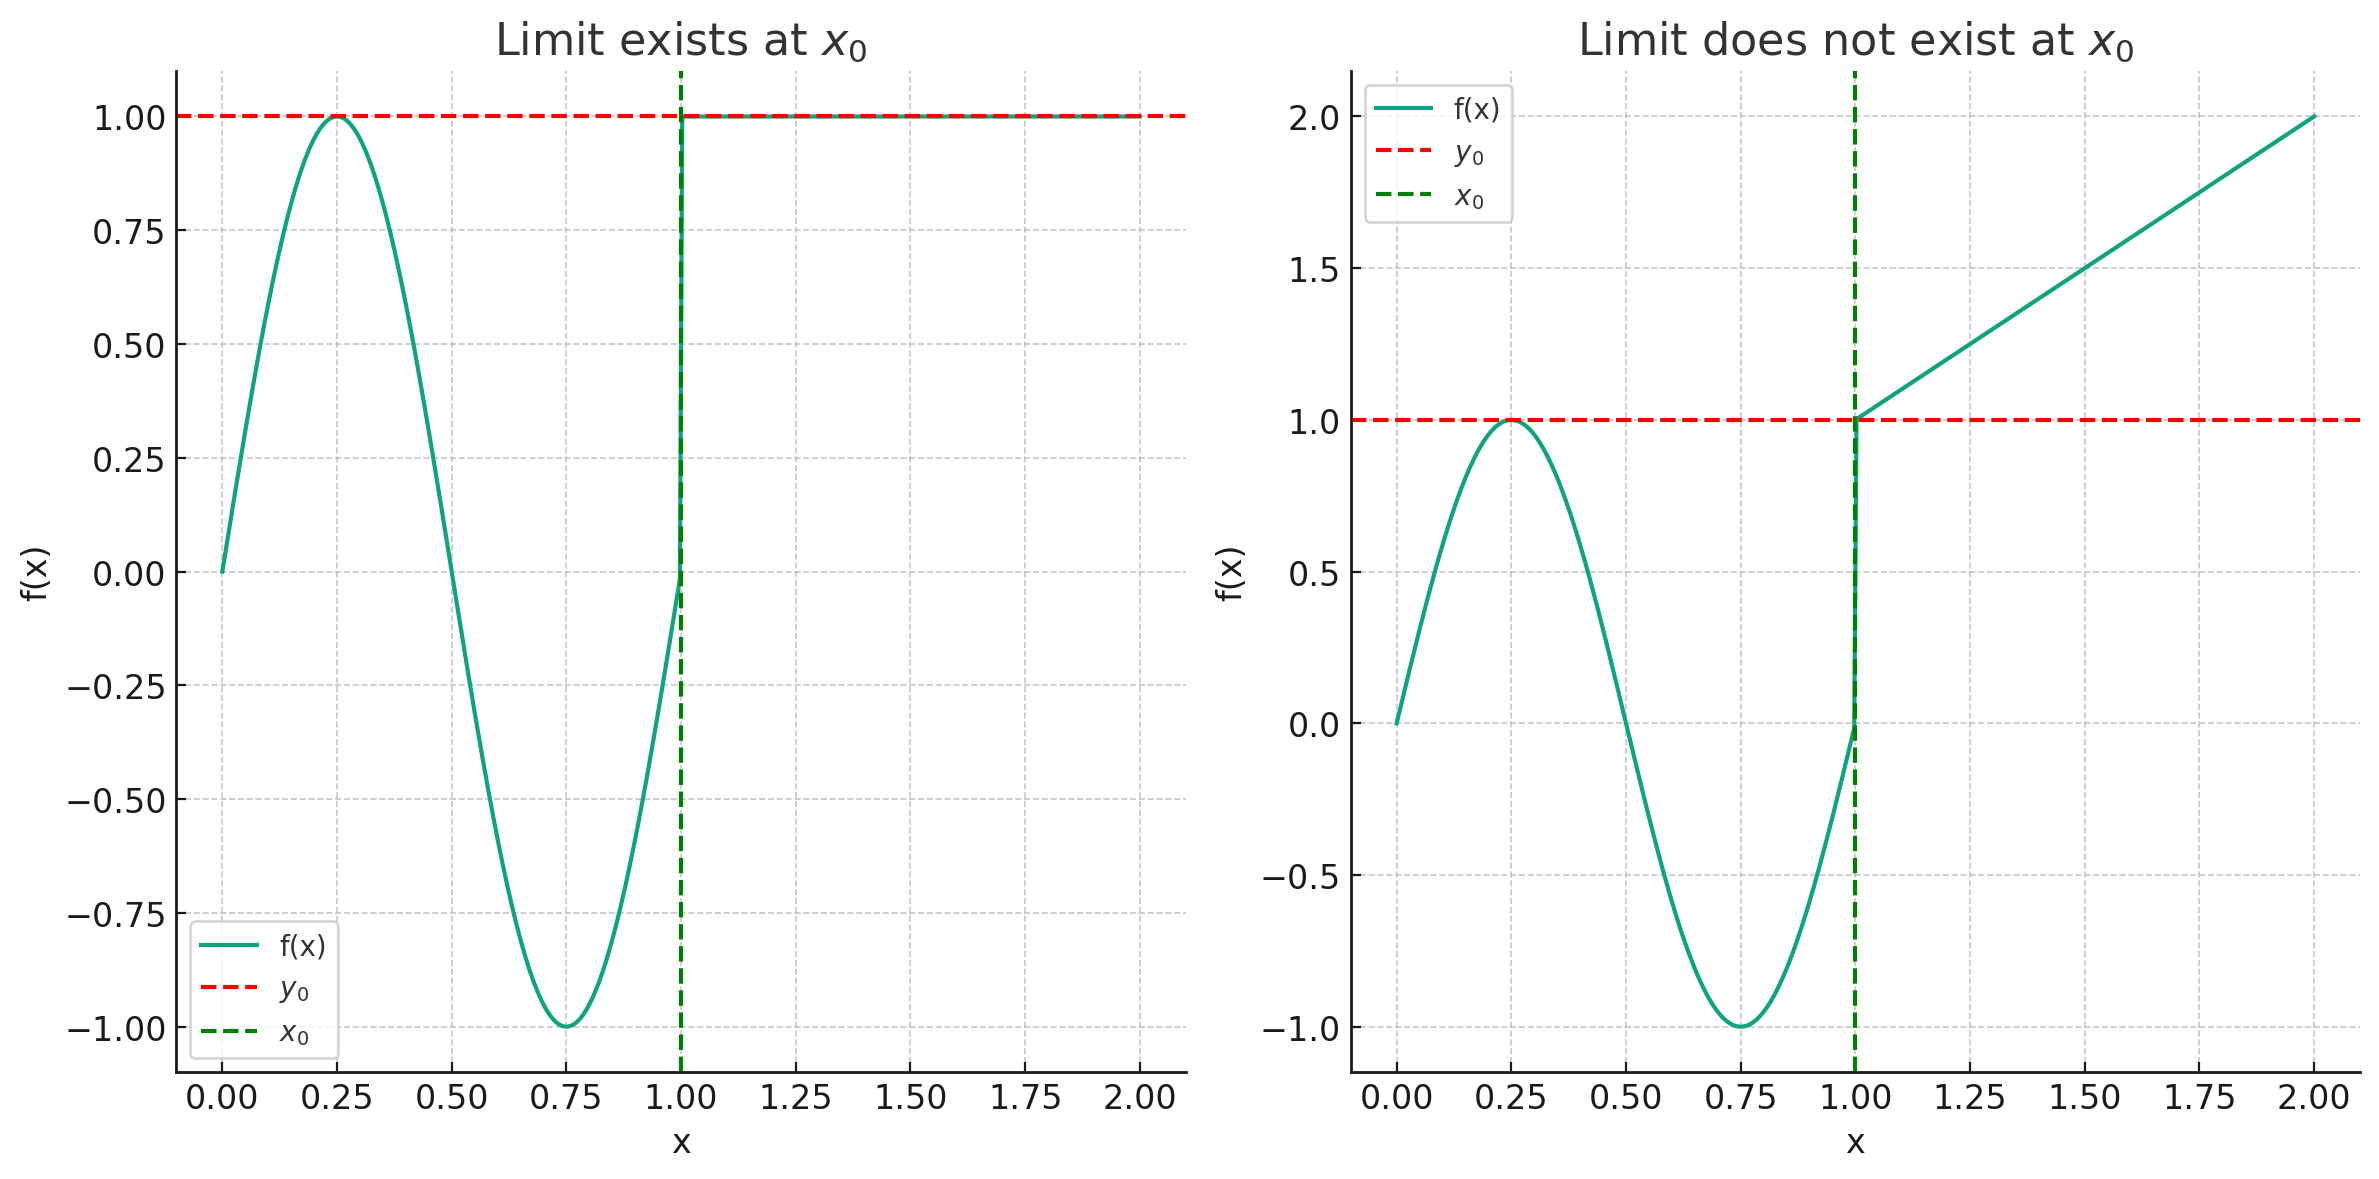
\includegraphics[width=1\textwidth]{img:grenzwertbegriff.png}

    \subsection{5 Beispiele zum Grenzwertbegriff}
        \begin{enumerate}
            \item $f(x) = \frac{\sin x}{x}, \quad x \not = 0$ \\ 
            Was ist $\lim_{x \to 0} f(x)$?
            \begin{multicols}{2}
                $\lim_{x \to 0} f(x) = 1$
                
                \columnbreak
            
                % Adjust the width as necessary
                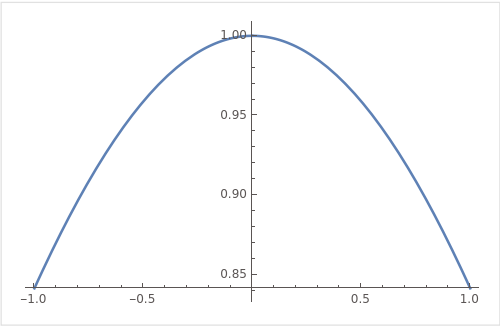
\includegraphics[width=0.5\textwidth]{img:5bsp-1.png}
            \end{multicols}
            
            
            \item $f(x) = \frac{\sin x}{x^2}, \quad x \not = 0 $ \\ 
            Was ist $\lim_{x \to 0} f(x)$?
            \begin{multicols}{2}
                
                $\lim_{x \to 0} f(x)$ \color{red} existiert nicht \color{black} 
                \columnbreak

                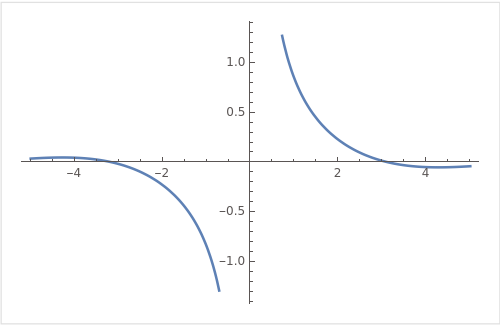
\includegraphics[width=.5\textwidth]{img:5bsp-2.png}
            \end{multicols}
            
            

            \item $f(x) = \frac{\sin x}{\left|x \right|}, \quad x \not = 0$ \\
            Was ist $\lim_{x \to 0} f(x)$?
            \begin{multicols}{2}
                
                $\lim_{x \to 0} f(x)$ \color{red} existiert nicht \color{black} 

                \columnbreak

                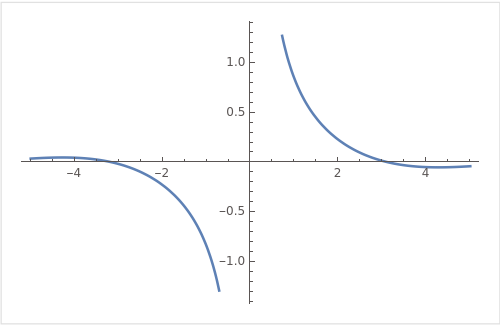
\includegraphics[width=.5\textwidth]{img:5bsp-2.png}

            \end{multicols}
            
            \pagebreak

            \item $f(x) = \sin \frac{1}{x}, \quad x \not = 0$ \\
            Was ist $\lim_{x \to 0} f(x)$?

            \begin{multicols}{2}
                
                $\lim_{x \to 0} f(x)$ \color{red} existiert nicht \color{black} 

                \columnbreak

                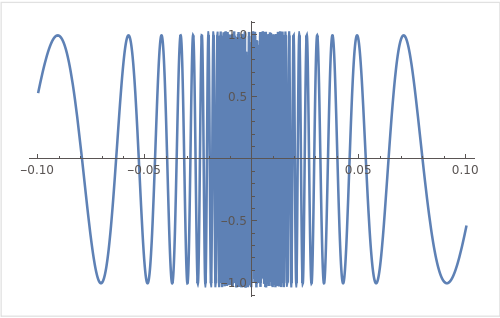
\includegraphics[width=.5\textwidth]{img:5bsp-4.png}

            \end{multicols}

            \item $f(x)= x \cdot \sin \frac{1}{x}, \quad x \not = 0,$
            Was ist $\lim_{x \to 0} f(x)$?

            \begin{multicols}{2}
                
                $\lim_{x \to 0} f(x) = 0$ 

                \columnbreak

                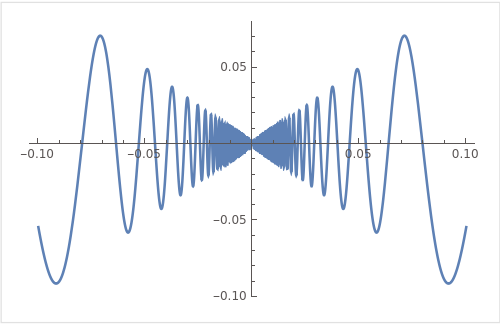
\includegraphics[width=.5\textwidth]{img:5bsp-5.png}

            \end{multicols}
        \end{enumerate}

        \begin{definition}[Linksseitige / rechtsseitige Grenzwerte  \\] 
        \begin{multicols}{2}
            $ \lim_{{x \to x_0}^+}f(x)$ \\ 
        $Y_0 = \lim_{{x \to x_0}^+} \text{Wenn}$
        $\forall \epsilon  > 0 : \exists b > 0 : $ fuer alle x mit $\left| x-x_0 \right| < b$ und $x > x_0$ gilt $\ldots $    
       \columnbreak
       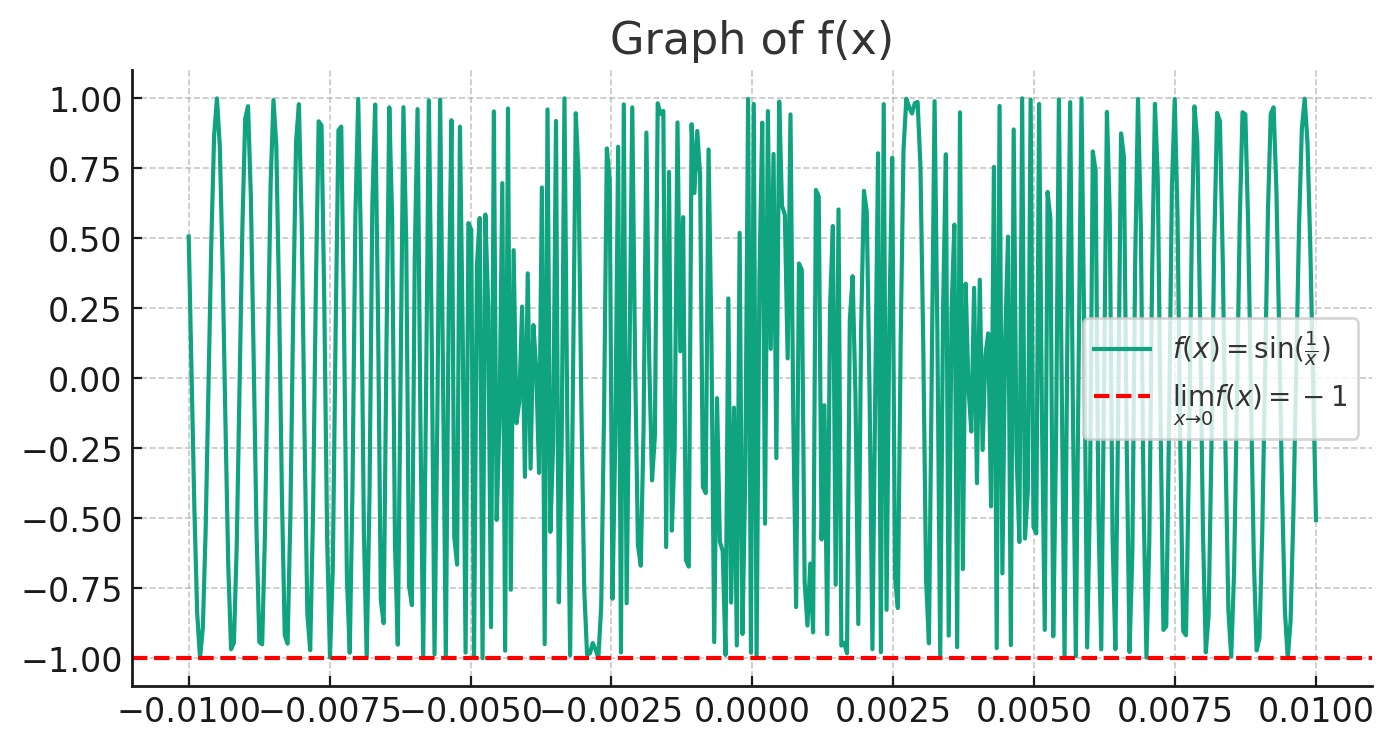
\includegraphics[width=0.5\textwidth]{3.6.2.png}
        \end{multicols}
    \end{definition}
        

        \begin{definition}[3.6.3 \\]
            \begin{multicols}{2}
                \( y_0 = \lim_{{x \to + \infty}} f(x) \) \\ wenn \( \forall \epsilon > 0: \exists M: \) \\ Immer wenn \( x > M \) , \\ dann gilt \( \left| f(x) - y_0 \right| < \epsilon \)

                \columnbreak

                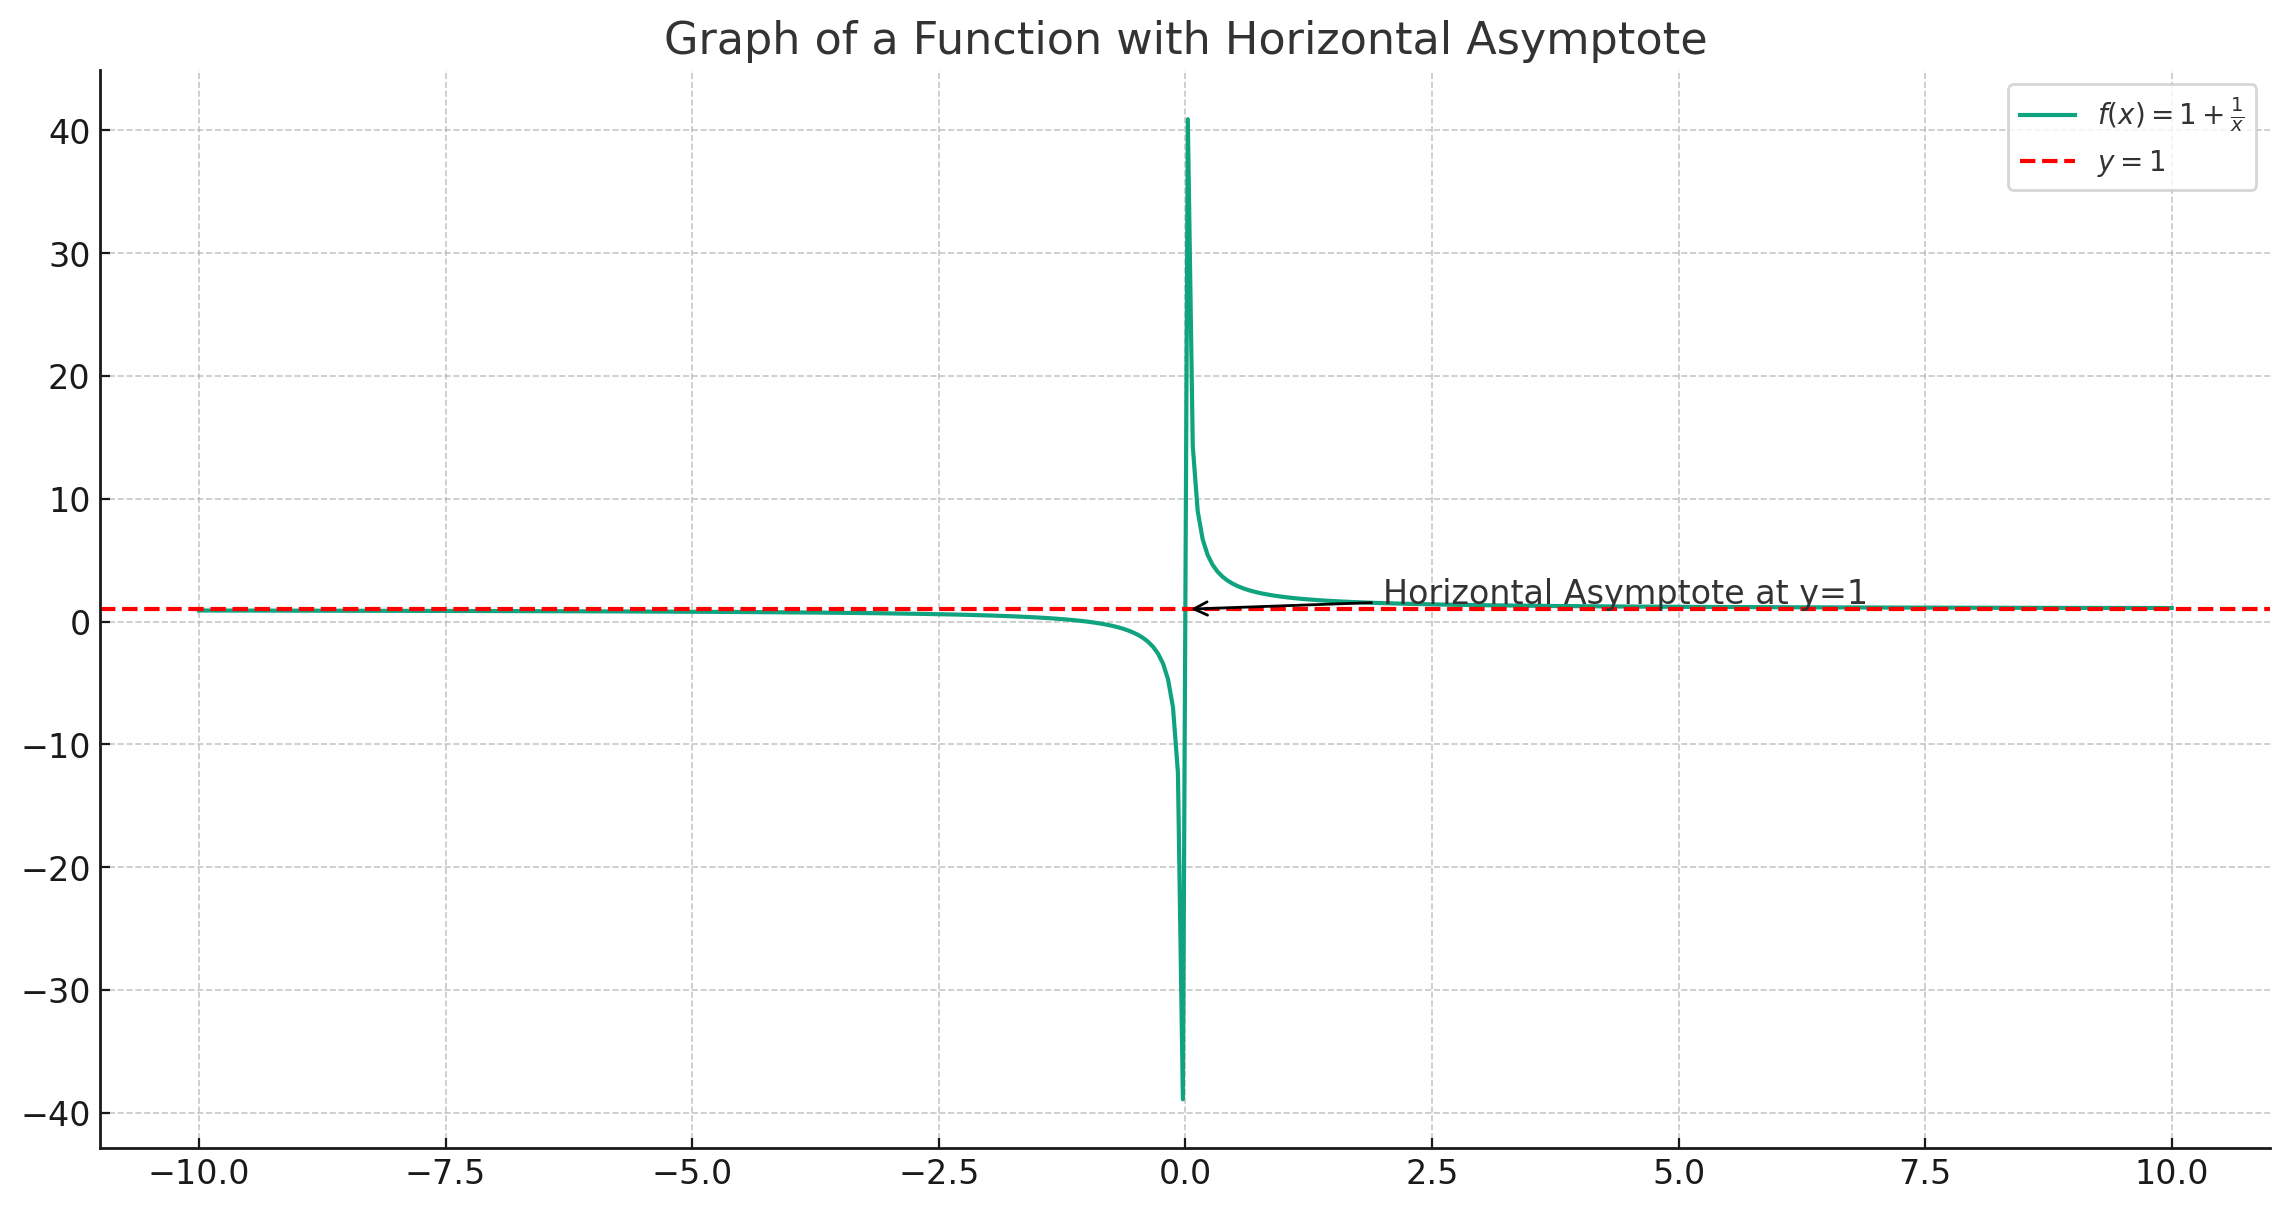
\includegraphics[width=0.5\textwidth]{3.6.3.png}
            \end{multicols}
        
        \end{definition}

        \begin{definition}[3.6.4 \\ ]
        $f$ heisst differnzierbar, in einem Punkt $x_0$ wenn der Grenzwert \\ 
        $\lim_{x \to x_0} \frac{f(x)-f(x_0)}{x-x_0} $  existiert. \\ 
        \bigskip
        Falls der Grenzwert existiert, schreibt man \textbf{dif:} $f^`(x_0)$ 
        \textit{Eine andere Schreibweise:} $\lim_{k \to 0} \frac{f(x_0+h) 0 f(x_0)}{k} $ 
            
        \end{definition}

        % Include Graphic
        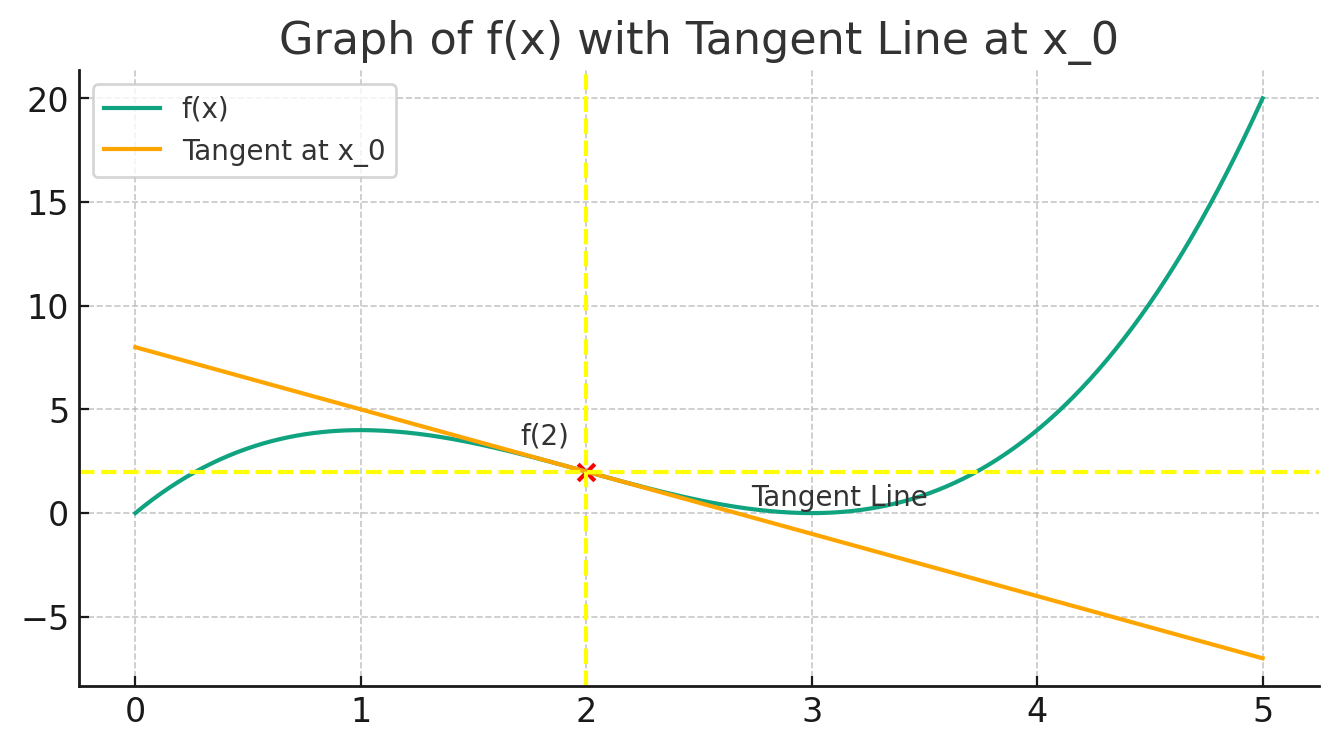
\includegraphics[width=1\textwidth]{3.6.4-tangente.png}
        Tangentengleichung: $g(x) = f(x_0) + \underbrace{f^`(x_0)}_{\text{Steigung der Funktion}} \cdot (x-x_0)$ r

    \section{Konversatorium 2023-11-21: \textbf{Ableitungen}}

    Potenzreihe $\sum_{k=0}^{\infty } a_k (x-\underbrace{x_0}_{\text{fix. meistens $x_0 = 0$}})^k$ \\ 
    Ist das \textbf{konvergent} Quotientenkriterium: 
    \[
    \limsup_{k \to \infty } \left| \frac{a_{k+1}(x-x_0)^{k+1}}{a_k(x-x_0)^k} \right| = \left| \overbrace{\left| x-x_0 \right| \cdot \limsup _{k \to \infty } \left| \frac{a_{k+1}}{a_k} \right|}^{\text{Ist das < 1 ?}} \right|
    \]
    Konvergent wenn $\left| x- x_0 \right| < \underbrace{\frac{1}{\limsup _{k \to \infty } \left| \frac{a_{k+1}}{a_k} \right|}}_{\text{Konvergenzradius $R$}}$
    Wenn $\limsup = + \infty \Rightarrow \quad R = 0$. \\ 
    Wenn $\limsup = 0 \quad \Rightarrow R = + \infty $, die \textbf{Potenzreihe} ist fuer alle x konvergent. \\
    
    \bigskip

    \subsection{Beispiel 1 Zu Konvergenzradius}
    $\sum_{k=0}^{\infty } k^k \cdot x^k$ Konvergenzradius $= \frac{1}{\limsup _{k \to \infty } \left| \frac{a_{k+1}}{a_k} \right|}$ \\ 
    \[
        \limsup _{k \to \infty } \left| \frac{(k+1)^{k+1}}{k^k} \right|  
        = \limsup _ {k \to \infty } \left| \frac{(k+1)}{k^k} (k+1)\right| = + \infty \quad R = 0 
    \]  
    Fuer kein $x \not = x_0 $ konvergent. 

    \subsection{Beispiel 2 Zu Konvergenzradius}

    \[\sum_{k=1}^{\infty } \frac{k!}{k^k} \cdot x ^ {k}
    \]
    Ich betrtachte $\limsup $ 
    \[
        \limsup_{k \to \infty} \left| \frac{\frac{(k+1)!}{(k+1)^{k+1}}}{\frac{k!}{k^k}} \right|
        = \limsup_{k \to \infty} \left| \frac{k^k \cdot (k+1)!}{(k+1)^{k+1} \cdot k!} \right|
        = \limsup_{k \to \infty} \left| \frac{k^k \cdot (k+1)}{(k+1)^{k+1}} \right|
        = \limsup_{k \to \infty} \left| \frac{1}{\left(\frac{k+1}{k}\right)^k} \right|
        = \frac{1}{e}
    \]
    
    Konvergenzradius $R = e$. 

    \bigskip

    \subsection{Definitionen zu Konvergenzradius}

    $e^x = \sum_{k=0}^{\infty } \frac{x ^ {k}}{k!}$, $\cos x = \frac{e ^ {ix} + e ^ {-ix}}{2}$, $\sin x = \frac{e ^ {ix} - e ^ {-ix}}{2i}$  \\
    Komplexe Zahl $z = a + ib$ \\ 
    Dann ist : $ \frac{z + \vec{z}}{z} = \frac{a+ ib + a - ib }{2} = \frac{2a }{a} = a - Re \quad z$ . \\ 
    Dann ist $\frac{z - \vec{z }}{zi } = \frac{a + ib - (a - ib ) }{2i} = b - $ 

    \bigskip

    \begin{multicols}{2}
        $e ^ {x + y } = e ^ {x} \cdot  e ^ {y } $, fuer alle x, y \\ 
        $\Rightarrow  e ^ {x } > 0 $ fuer alle $ x \in \mathbb{R}$ \\ 
        $e ^ {-x } = \frac{1}{e ^ {x}}$  fuer alle $x \in \mathbb{R}$ \\
        Exponentialfunktion ist \textbf{bijektiv } $\mathbb{R} \rightarrow \mathbb{R ^ {+ }}$ \\ 
        $\sin $ und $\cos $ sind periodisch mit \color{red} reeller \color{black} Periode $2 \pi $ \\
    
        \columnbreak

        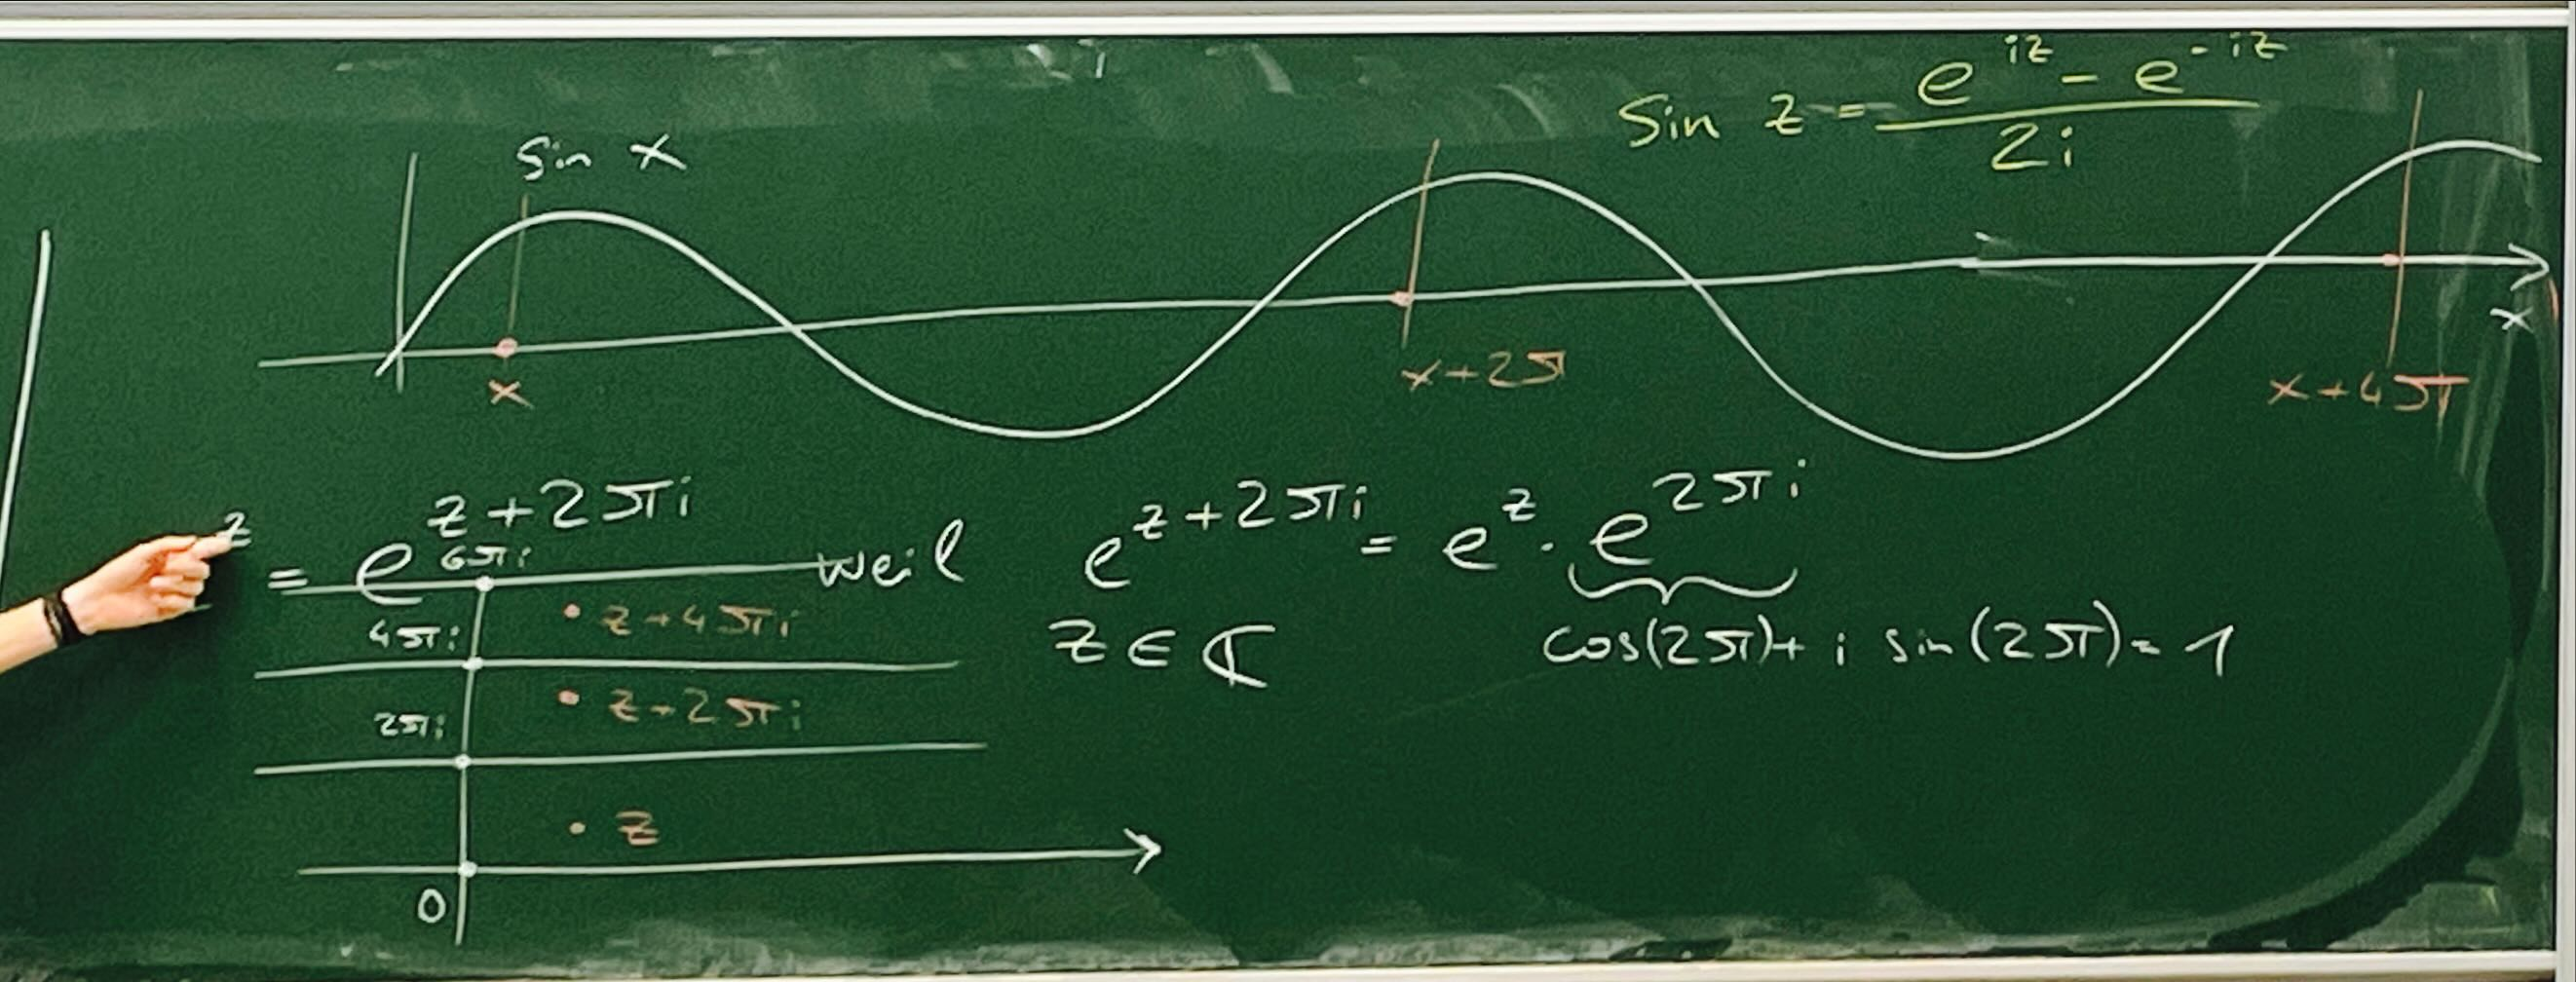
\includegraphics[width=.5\textwidth]{img:konversatorium202311210944.jpeg}
    \end{multicols}

    \bigskip

    \subsection{Definition zum Logarythmus}

    \begin{multicols}{2}
        $\ln: \mathbb{R ^ {+}} \leftarrow \mathbb{R}$ \\ 
        Was heisst $\ln  y$?  \\ 
        \textit{Ein Ding das ich in die Exponentialfunktion einsetzen kann so dass} $e ^ {\text{Ding}} = y$ \\ 
        Was ist $\ln a + \ln b$? 
        
        \[
            e ^ {(\ln a + \ln b)} = e ^ {\ln a} \cdot e ^ {\ln b} =  a \cdot b = e ^ {(\ln (a b))}
            \Rightarrow \color{red} \ln (a \cdot b) = \ln a + \ln b \color{black}
        \]
        \columnbreak

        \[e ^ {x} = y \]
        \[x = \ln y\]
    \end{multicols}
    
    \bigskip

    Wir wissen $e ^ {2x} = e ^ {x + x} = e ^ {x} \cdot e ^ {x } = (e ^ {x}) ^ {2}$ \\ 
    $\vdots$  
    \begin{multicols}{2}
        Was ist $ln(a ^ {b})$
        \[
            e ^ {(\ln a ^ {v})} \Rightarrow  \color{red} \ln (a ^ {b}) = b \cdot \ln a \color{black}
        \] 

        \columnbreak

        \[
            ln (2 ^ {100} ) = 100 \cdot \underbrace{\ln (2)}_{\approx 0,61} \approx 61
        \]
        Wie gross ist $2 ^ {100}$ ungefaehr ? Ungefaehr $e ^ {61}$ 
        \[
            b \ldots  \text{Basis } > 0
        \]
        \begin{definition}[Logarythmus]
            \[\log_{b} x = \frac{\ln x}{\ln b} 
    \]
        \end{definition}
    \end{multicols}
    
    \section{Konversatorium 2023-11-28: \textbf{Funktionen}}

    \subsection{Rechenbeispiel 1}
    Given the function:
\[ f(x) = 2x^3 - 3x^2 - 12x + 8 \]
for the interval \([0, 4]\), we first find its derivative:
\[ f'(x) = 6x^2 - 6x - 12 \]

To find the critical points, we solve for \(x\) in the equation \(f'(x) = 0\):
\[ 6x^2 - 6x - 12 = 0 \]

This can be simplified to:
\[ x^2 - x - 2 = 0 \]

Solving this quadratic equation, we get the critical points:
\[ x_{1,2} = \frac{-(-1) \pm \sqrt{(-1)^2 - 4 \cdot 1 \cdot (-2)}}{2 \cdot 1} = \frac{1 \pm \sqrt{9}}{2} = \left\{ 2, -1 \right\} \]

However, since we are considering the interval \([0,4]\), only \(x = 2\) is relevant.

Now, evaluating \(f(x)\) at 0, 2, and 4:
\[ f(0) = 8 \]
\[ f(2) = 2 \cdot 2^3 - 3 \cdot 2^2 - 12 \cdot 2 + 8 = -12 \]
\[ f(4) = 2 \cdot 4^3 - 3 \cdot 4^2 - 12 \cdot 4 + 8 = 40 \]

% Assuming you have an image named "Bildschirmfoto 2023-11-28 um 9.15.57 AM.png" in the "img" folder
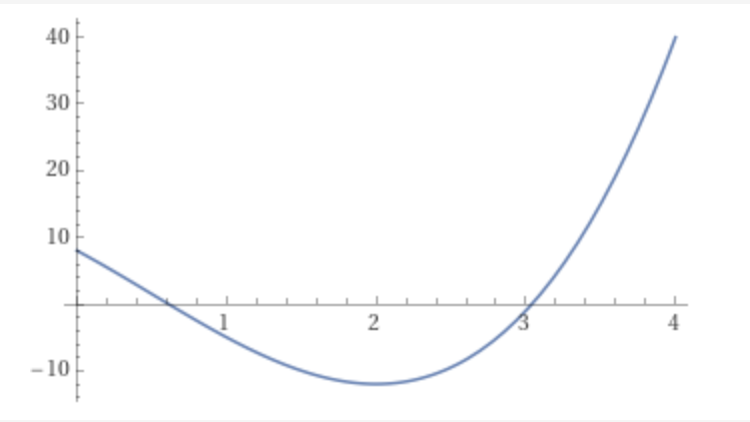
\includegraphics[width=10cm]{img/Bildschirmfoto 2023-11-28 um 9.15.57 AM.png}

\subsection{Rechenbeispiel 2}
Given the function:
\[f(x) = e^x (2x^2 - 3 x + 1) \text{fuer} x \in [-1,2]\]
we first find its derivative:
\[\ldotp\]
Solving this quadratic equation, we get the critical points:
\[f(-1) = \frac{6}{8} = 2,2\]
\[f(\frac{-1 \sqrt{17}}{4}) = -0.27\]
\[f(2) = 3 e ^ {2} \approx 22,17\]
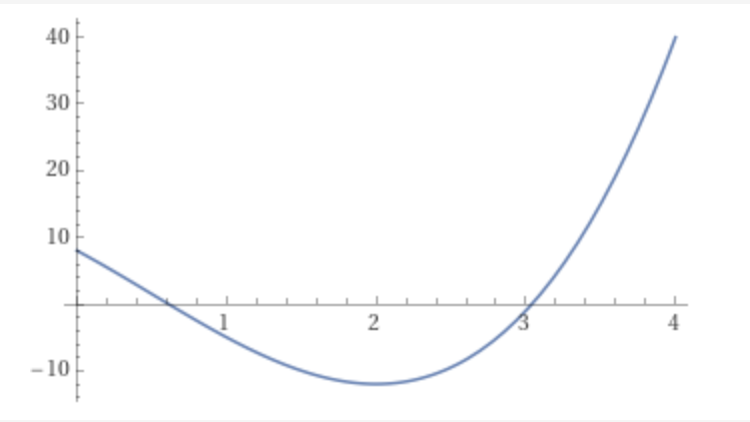
\includegraphics[width = 10cm]{img/Bildschirmfoto 2023-11-28 um 9.15.57 AM.png}

\subsection{Rechnebeispiel 01 zur Regel von L'Hospital}
\begin{theorem}[Regel von L'Hospital]
    Seien $f,g: I \rightarrow \mathbb{R}$ differenzierbar mit $g(x) \not = 0$ für alle $x \in I$ und $x_0 \in I$ mit $\lim_{x \to x_0} f(x) = \lim_{x \to x_0} g(x) = 0$ oder $\lim_{x \to x_0} g(x) = \pm \infty$. Dann gilt:
    \[\lim_{x \to x_0} \frac{f(x)}{g(x)} = \lim_{x \to x_0} \frac{f'(x)}{g'(x)}\]
\end{theorem}

    \[\lim_{x \to 0} \frac{e ^ {2x}-1 - 2x}{x ^ {2}} = \frac{0}{0}\]
    Find it's derivative:
    \[\lim_{x \to 0} \frac{2e ^ {2x} - 2}{2x} = 2 \cdot 1 = 2\]
    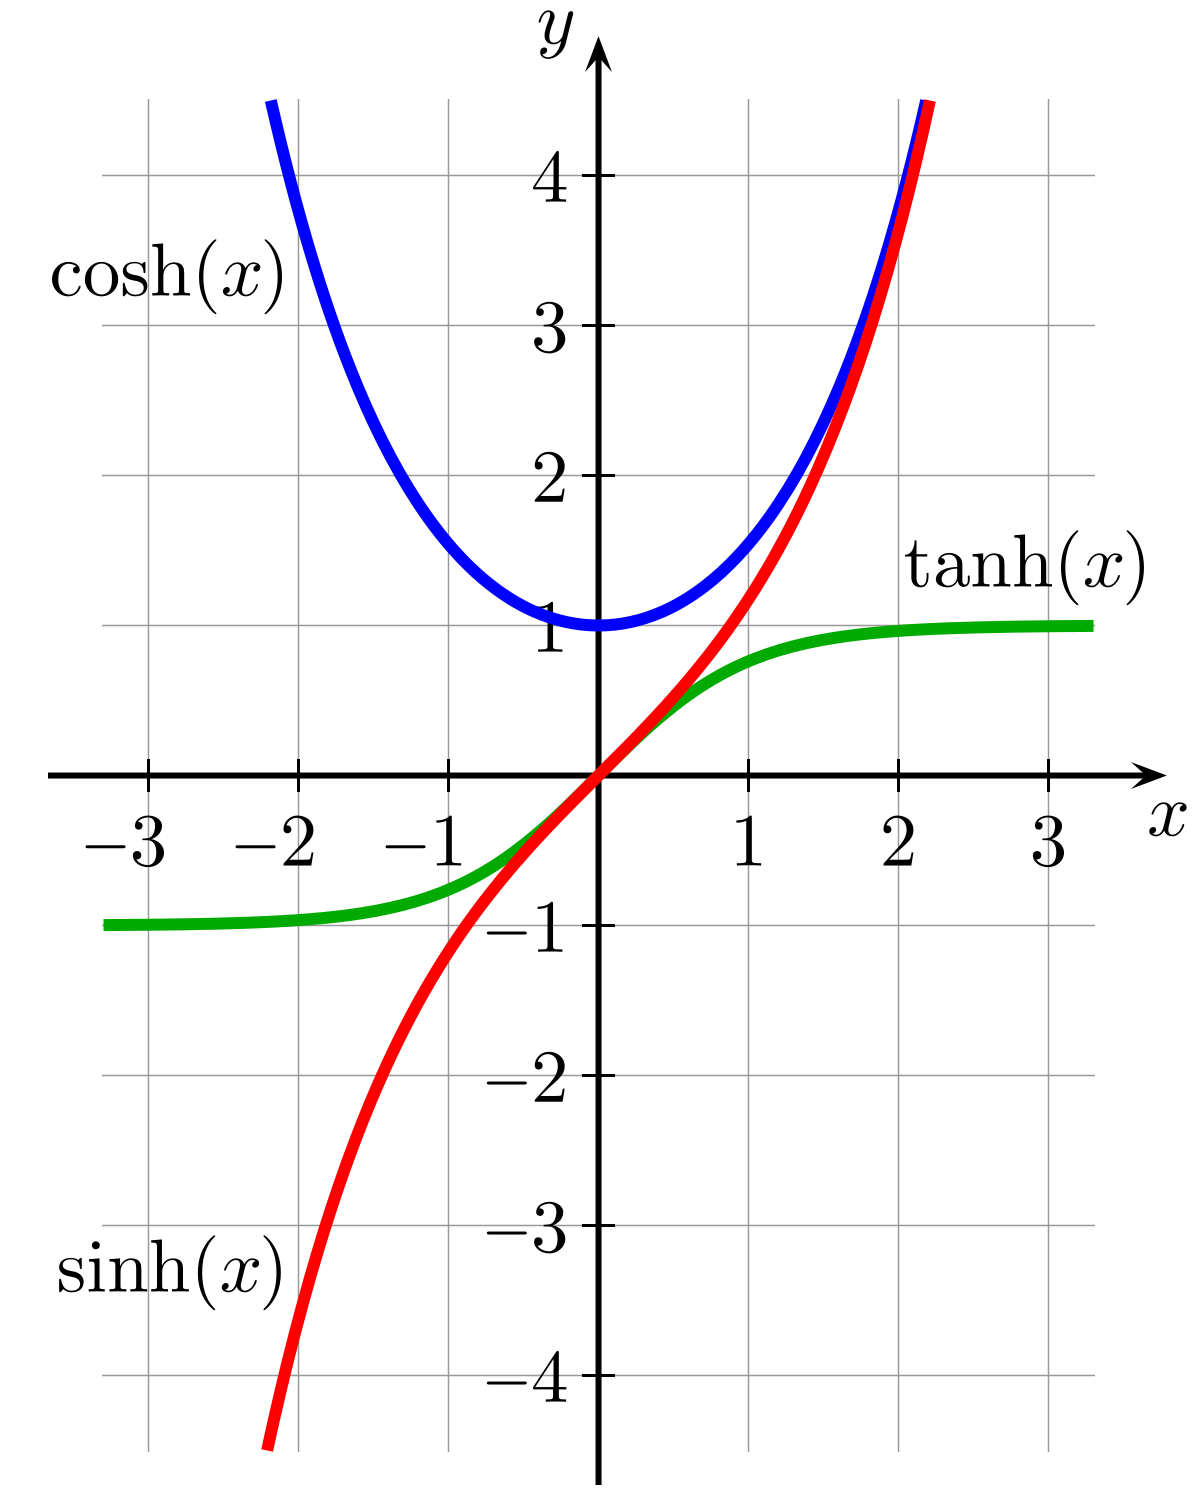
\includegraphics[width = 10 cm]{1200px-Sinh+cosh+tanh.svg.png}
    \[= \frac{2}{2} = 1\]


\subsection{Rechnebeispiel 02 zur Regel von L'Hospital}
\[\lim_{x \to 0} \frac{\sinh (x) + \sin (x)}{\sin (x) + x\cos(x)}\]

\end{document}